\documentclass{article}
\usepackage{graphicx}
\usepackage{amssymb}
\usepackage{amsmath}
\usepackage{eurosym}
\usepackage{fullpage}
\usepackage{multirow}
\usepackage{fancyhdr}
\usepackage{amsmath}
\pagestyle{empty}
\usepackage{placeins}
\usepackage{changepage}
\usepackage[dvipsnames]{xcolor}
\usepackage{collectbox}
\usepackage{wrapfig}
\usepackage[utf8]{inputenc}
\usepackage[english]{babel}
\usepackage{gensymb}
\usepackage{tikz}
\usepackage{pgfplots}
\usepackage{graphicx}
\usepackage{booktabs}
\usepackage{enumitem}
\usepackage{afterpage}
\usepackage{overpic}
\usetikzlibrary{calc}
\usetikzlibrary{calc,patterns,angles,quotes}
\usepackage{xfrac}
\usetikzlibrary{automata, positioning}
\usepackage{color,soul}


\pgfplotsset{width=9cm,height=6.5cm,compat=1.9}

\setcounter{page}{1}


% Alternate method of doing solution function.
%\newcommand{\sol}[1]{}
%\renewcommand{\sol}[1]{{\color{blue} #1 \fi}}

%----------------------------------COMMANDS----------------------------------------------------
%---Create function to control text solution display----------------%
\newif\ifPrintSolution
\newcommand{\showSolution}{\PrintSolutiontrue}
\newcommand{\sol}[1]{\ifPrintSolution {\color{blue} #1 } \fi}
%---END Solution Function-------------------------------------------%

%---Create function to control R-Code solution display--------------%
\newcommand{\solR}[1]{} 
%---END R-Code Solution Function------------------------------------%

%%%%%%%%%%% Turn ON/OFF text solutions with this command%%%%%%%%%%%
\showSolution % comment out to hide solutions 
%%%%%%%%%%% Turn ON/OFF R-code solutions with this command%%%%%%%%%
\renewcommand{\solR}[0]{} % Comment out to hide R-Code Solutions

%------------------------------------------------------------------------------------------------

% Use \sol for text solutions and \solR for code chunk solutions


\begin{document}

\noindent \textbf{MA206  Lesson 2 - Preliminaries}
\vspace{.1in}

\textbf{Understand the 6-Step Process}

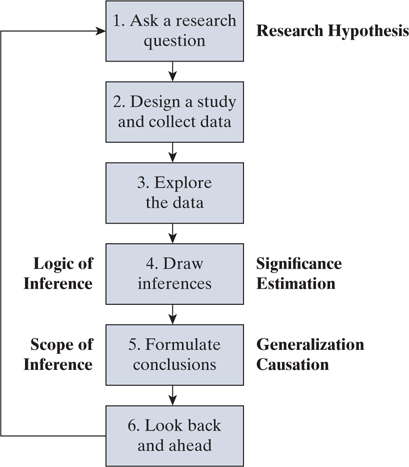
\includegraphics[scale=0.6]{6_Step_Process.png}

\vspace{0.25in}

\textbf{Understand how to visually interpret the data}\\

\hspace{0.1in} \textbf{Shape}

\sol{We want to look if the distribution is symmetric, where it is centered, and how many peaks there are.}
\vfill

\hspace{0.1in} \textbf{Center}

\sol{Where is the distribution centered on? What is a typical value?}
\vfill

\hspace{0.1in} \textbf{Variability}


\sol{How spread out or concentrated is the data? We often report this variation through \textbf{standard deviation}, which can be crudely explained as the average distance of our data from its mean}
\vfill

\hspace{0.1in} \textbf{Unusual Observations}

\sol{Are there \textbf{outliers} which are very different from most observations? Can this difference be explained? Could it be entered in error?}
\vfill

\pagebreak

Looking forward, we want to look at a housing market to buy our house to live in. This could be your first duty station near a military base, or your retirement home in the perhaps not so distant future. You want to buy, but are unsure what you should spend. Think of a location and explore using data.

\section*{1: Ask a Research Question}

What is your research question?

\vspace{0.5 in}

\section*{2: Design a Study and Collect Data}

We will utilize redfin.com to collect the data from our analysis. Download the .csv file for your area and save it into your working directory to load it into R.

What are the \textbf{observational units}?

\vspace{0.25 in}

Give some examples of notable \textbf{variables of interest} and categorize them as either quantitative or categorical.

\vspace{0.5 in}


\section*{3: Explore the Data}

Describe the \textbf{distribution} of the prices of the houses in your area of interest

\textbf{Shape}\\

\textbf{Center}\\

\textbf{Variability}\\

\textbf{Unusual Observations}


\vspace{0.5 in}

What is the mean and standard deviation of the housing prices in your area?

\vspace{1.5 in}


Conduct further data exploration and annotate any interesting findings or charts.

\vfill

\newpage

\section*{4: Draw Inferences}

We will get into \textbf{Draw Inferences} throughout the course to build tools to indicate if there is an effect between variables. For example, we might provide evidence that as a home's square footage increases, the sales price increases. What else might we wish to infer?

\vspace{0.5 in}

\section*{5: Formulate Conclusions}

To what underlying process or larger group can these conclusions be generalized? Again, we will get further into \textbf{Formulate Conclusions} throughout the course, but here we would not apply the conclusions from our analysis outside the houses in the local area because that is all our \textbf{sample} is from. What generalizations or causations can we infer from our data?

\vspace{0.5 in}

\section*{6: Look Back and Ahead}

We could identify limitations of our study, such as the limited region of houses looked at. For example, there could be interactions between the variables, another tool we will explore later in this course.  For future research, there are probably other factors not captured in Redfin housing data that impacts housing costs - for example, as Clermont is in Lake County, a "water front property" status could impact prices in a way that is not captured in our analysis. 

\end{document}
